\chapter{p-p Interactions and their Simulation}
\label{chap:event:MC}

\section{p-p Interactions and Parton Distribution Functions}

The partonic center of mass energy \cmpart is lower than the total center of mass energy.

\subsection{Factorization Theorem}



\begin{figure}[h]
\begin{center}
%  \subfigure[]{
%    \label{fig:Comb_syst:pt}
    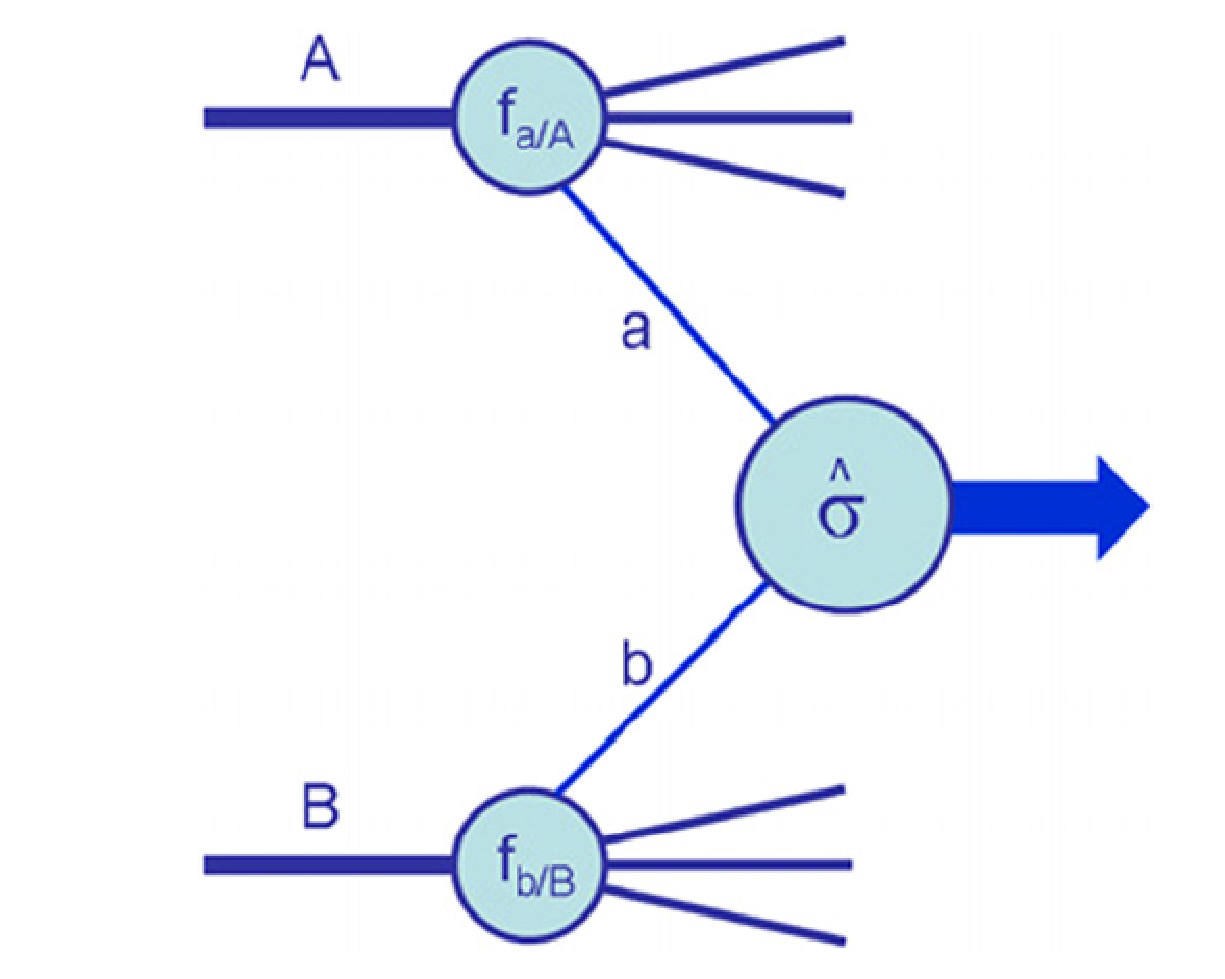
\includegraphics[width=0.58\textwidth]{figures/simul/ppcoll}
%  }
\end{center}
 \caption{Diagrammatic structure of a generic hard-scattering process. Figure from Ref. \cite{Campbell:2006wx}.}
  \label{fig:sim:pp}
\end{figure}

\subsection{Parton Density Functions}

\begin{figure}[h]
\begin{center}
    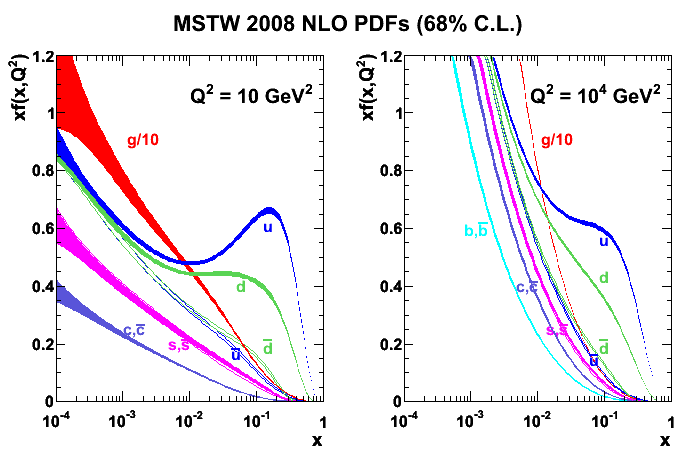
\includegraphics[width=0.8\textwidth]{figures/simul/pdf}
\end{center}
 \caption{MSTW 2008 NLO PDFs at Q$^2$ = 10 GeV$^2$ and Q$^2$ = 104 GeV$^2$. Figure from Ref. \cite{Martin:2009iq}.}
  \label{fig:sim:pp}
\end{figure}


\section{Generation of the Events}

\subsection{Matrix Element}

\subsection{Parton Shower}

\subsection{Matching}

\subsection{Hadronization}

\section{MC Generators}

\section{Detector Simulation}

\section{Data-driven Corrections}
